\chapter{Results\label{ch:results}}

Table B.1 shows estimates for models (4.6), (4.7) and (4.8) implemented via the probit specification. Significant coefficients for demographic variables, economic conditions, as well as industry effects were reported for different levels of $\alpha$. The total probit model estimates a negative coefficient $\beta_{female} = -0.204$, statistically significant at the $\alpha = 1\%$ level and among the biggest in magnitude across covariates. This proves the need to investigate how the probability to enter entrepreneurship differs for men and women, and what factors matter for each group.

\section{Demographic variables}

\begin{figure}[hbtp]
	  \centering{%
		  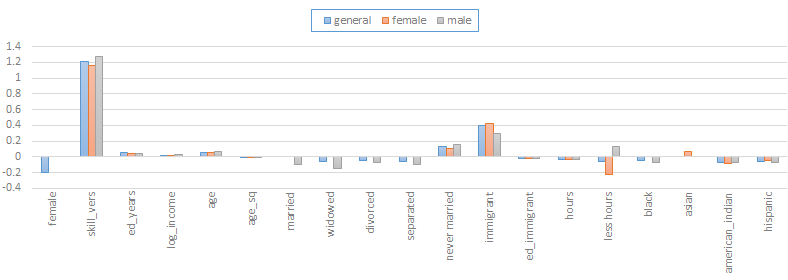
\includegraphics[width=1\linewidth]{ch-results/individual.png}%
    	}%
    \caption{Magnitude of Significant Coefficients for Individual Level Variables} 
\end{figure}

Figure 5.1 illustrates the magnitude of significant coefficients comparatively across the three models for variabes that pertain to the agent-level. We note that for covariates like skill diversification or immigrant status, the three estimates are fairly consistent in magnitude and sign, while variables like $less\_hours$, the number of hours associated with the transition to self-employment, have differential effects on men and women. 

\subsection{Education}

Educational attainment is one of the most significant demographic factors to affect entry decisions, with a positive coefficient $\beta_{ed} = 0.0497$ for the entire dataset, a similar value for women, $\beta_{ed} = 0.0482$ and a smaller effect for men, $\beta_{ed} = 0.0418$. The F statistic testing the equality of the coefficients shows a significant difference across genders, with a greater magnitude for the effect of female educational attainment. 

The interaction term for skill level and immigration status also provides important insights as to how education affects entrepreneurship decisions. While immigrant status is positively associated with likelihood of self-employment entry, with $\beta_{immigr} = 0.427}$ for women and $\beta_{immigr} = 0.291$ for men, this control has negative effects when interacted with years of education. In this case, the overall coefficient is $\beta_{ed*immigr} = - 0.0240$, with a stronger negative effect for women ($\beta_{ed*immigr} = - 0.0254$) than for men ($\beta_{ed*immigr} = - 0.0163$). 

Education also factors in when interacted with GDP change at the state level, causing differential effects for periods of economic upturn and downturn.  Here, men record a negative coefficient $\beta_{ed*econ} = -0.00126$, meaning that in times of economic upturn (positive GDP change), a higher number education years makes it less probable for them to start a business. For women, this hypothesis does not hold, with the interaction between education and GDP change having a positive coefficient $\beta_{ed*econ} = 0.00142$. For periods of economic upturn, higher education for this group translates to a higher probability for business entry. 

\subsection{Skill Versatility}

An arguably related measure, an individual's skill versatility has a significant positive effect on the likelihood of self-employment, with the greatest magnitude among the covariates in Figure 5.1. To this regard, the coefficients are $\beta_{change} = 1.165$ for women and $\beta_{change} = 1.271$ for men, indicating a greater degree of flexibility leads to a higher probability of self-employment. The estimates are not significantly different across genders, and are in line with the results for the general sample, pointing to a robust effect of this factor on self-employment entry. 

\subsection{Age}

The coefficients on age describe a quadratic function with $\alpha <0 $, given $\beta_{age} = 0.0578$ and $\beta_{age^2} = -0.000534$ for the complete dataset. For women, these values are similar, with $\beta_{age} = 0.0578$ and $\beta_{age^2} = -0.000534$, while for men they are greater in magnitude, with $\beta_{age} = 0.0629$ and $\beta_{age^2} = -0.000595$. The shape of the concave-down parabola implies a positive effect of age on self-employment until a maximum value is reached. For any value greater than this vertex, there is a negative effect of age on the probability of entry. These results are consistent for the data in the aggregate, as well as when differentiated by gender.

\subsection{Immigrant Status}

Immigrant status on its own also affects the probability of entry, with positive coefficients across all three groups. When not interacted with educational attainment, $\beta_{immigr} = 0.404$ for all data, with an estimate similar for women -- $\beta_{immigr} = 0.427$ and significantly lower for men -- $\beta_{immigr} = 0.291$. This gender difference is significant, as reported by our F test. When conditioned on years of education, the coefficient changes sign and magnitude, as we previously saw. 

\subsection{Marriage Status}

Marriage status was analyzed both on its own and in interaction with other factors. Being married was found to have a significant negative effect on men's self-employment entry, with $\beta_{married} = -0.954$. The effect on women is of opposing sign, with $\beta_{married} = 0.0259$ denoting a positive influence on the likelihood of transitioning into self-employment. At the other end, the coefficients on not having been married contradict previous research, with positive effects on the probability of starting a business across all groups ($\beta_{never\_married} = 0.112$ for women and $\beta_{never\_married} = 0.156$ for men). Here, gender differences are not observed, with equally positive effects on the probability of starting a business. When marriage status is instrumented with income or hours worked, we find no significance to the new coefficients, disproving the extent to which being married can affect monetary motivations or induce different work patterns for men and women.

\subsection{Race}

Race affects the probability of entry, with most minority groups having negative coefficient estimates for both genders. Being American Indian has the greatest negative effect on the probability of self-employment for the whole dataset, followed by being Hispanic and Black. Being Asian is here the only covariate with a positive effect on entry probability ($\beta_{asian} = 0.0439$). Differences in magnitude still exist between men and women, with black males having a significantly more negative coefficient than females ($\beta_{black\_male} = -0.0726$ versus $\beta_{black\_female} = -0.0196$), a pattern that holds for hispanics as well ($\beta_{hisp\_male} = -0.0755$ versus $\beta_{black\_female} = -0.0470$). At the other end, being an Asian woman has a greater positive coefficient than the male counterpart, with coefficient estimates $\beta_{asian\_female} = 0.0675$ and $\beta_{asian\_male} = 0.0083$ respectively. 

\section{Capital constraints}

In terms of the availability of capital, the level of family income at the first survey time is found to have a significant positive effect on the probability of self-employment, with a bigger coefficient for men ($\beta_{income} = 0.0260$) than women ($\beta_{income} = 0.0157$). This difference is significant when subjected to an F-test, and speaks to the important effect of capital in incentivizing business formation.

\section{Employment Characteristics}

Past employment characteristics are a telling covariate, with negative coefficients on hours worked at $t_0$ across groups. The estimates are $\beta_{hours} = -0.0377$ for women and $\beta_{hours} = -0.03893$, values that are not significantly different at the $\alpha = 1 \%$ level. The more an individual works at their current job, the less likely the transition into self-employment is, a finding that holds across genders.

Lifestyle changes vary in their power to incentivize business formation among men and women. The coefficient measuring the difference in hours between survey times denotes that among men, self-employment is positively affected by the promise of less hours worked ($\beta_{less\_hours} = 0.128$). For women, this is not the case, with $\beta_{less\_hours} = 0.128$. The prospect of working less has a negative impact on women's decision about business entry, a significantly different effect from their male counterparts. Contrary to expectations, the signs for these coefficients are not altered by marriage status, with no statistical significance for the associated interaction term. 

\begin{figure}[hbtp]
	  \centering{%
		  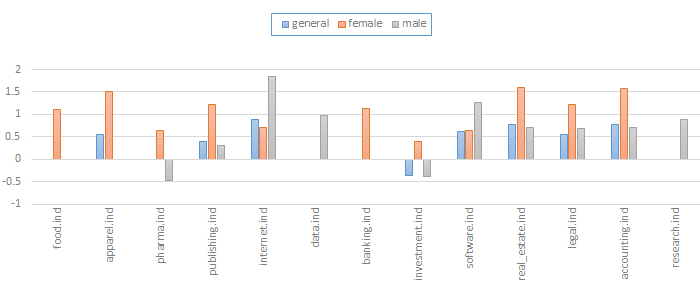
\includegraphics[width=1\linewidth]{ch-results/industry.png}%
    	}%
    \caption{Magnitude of Significant Industry Coefficients by Gender} 
\end{figure}

As illustrated by Figure 5.2, results also show consistent patterns of gender division across industries, with fields more traditionally occupied by men remaining prominent choices for new businesses for this group. The coefficients for men in tech industries are $\beta_{Data} = 0.967$, $\beta_{Software} = 1.259$ or $\beta_{Internet} = 0.967$. All the while, female self-employment is more positively incentivized by industries traditionally avoided by men, as indicated by $\beta_{Apparel} = 0.967$ or $\beta_{Accounting} = 1.575$ for the female sample.

It is important to note that both the male-dominated and female-dominated industries generate coefficients on men/women respectively that significantly surpass the values for the general sample [see Figure 5.2]. In that sense, the probit model for the data in the aggregate estimates an average effect of certain industries on probability of self-employment entry, one that misses the important asymmetries across genders. 

\section{Environment Variables}

\begin{figure}[hbtp]
	  \centering{%
		  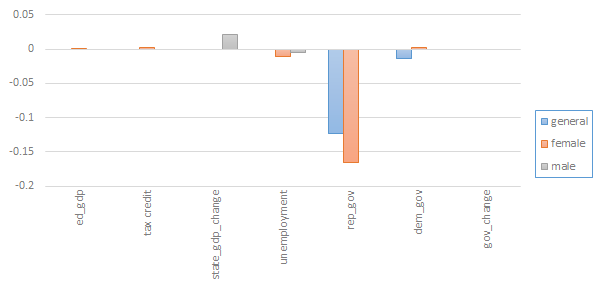
\includegraphics[width=1\linewidth]{ch-results/external.png}%
    	}%
    \caption{Magnitude of Significant Coefficients for Environment Variables} 
\end{figure}

Figure 5.3 plots significant coefficients for the external factors thought to affect an agent's decision to enter self-employment. Here, we note more pronounced effects of the gender split, with most covariates affecting men or women significantly, but not both groups. 

\subsection{Economic Conditions}

Unemployment is a significant indicator of how local economic conditions affect self-employment rates, with negative coefficients $\beta_{unemployment} = -0.0113$ for women and $\beta_{unemployment} = -0.00514$ for men. Although of the same sign, these values are found to differ in magnitude at the $\alpha = 1\% $ significance level, women being less likely to start a business when there is a high unemployment rate in their respective state. 

\subsection{Policy Climate}
Tax incentives for starting a business also show more significant responsiveness in the sample of female respondents, with  $\beta_{tax\_credit} = 0.0021$. For men, this coefficient is negative, $\beta_{tax\_credit} = -0.0131$, pointing to a reverse effect of tax credit on business formation. Instead of contributing to the likelihood of business formation, tax credits are estimated to have a negative effect for the male sample. This difference is significant at at the $\alpha = 1\% $ level. 

The party affiliation of state governors is found to matter differently across gender groups. Having a republican governor has a significant negative effect on business formation for women, with $\beta_{rep\_gov} = -0.165$, while having a democratic governor seems to have a slight positive effect on women's self-employment, with  $\beta_{dem\_gov} = 0.0017$. For the male sample, the effects are of opposite sign ($\beta_{rep\_gov} = 0.0775$ and $\beta_{rep\_gov} = -0.0103$), but not significant at the $\alpha = 5\% $ level. 

\section{Evaluation of Results}

The majority of reported coefficients are significant at the $\alpha = 5\% $ level, with some particular patterns for men and women. For covariates like being married or widowed, the effect seems to only be significant for men, while the interaction between GDP change and education level or local governance indicators hold more in the case of women. For the general model, $PseudoR^2 = 0.542$ for the general model, and similar values for men - $PseudoR^2 = 0.5328$ and women - $PseudoR^2 = 0.5595$. Although we are able to explain the highest degree of variability for the female sample, overall the regression models provide a good fit.























